\begin{figure}
    \centering
    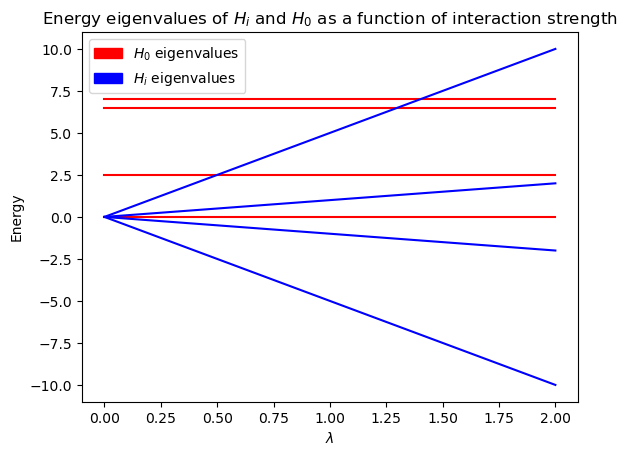
\includegraphics[scale=0.4]{figs/Eig_lmd.png}
    \caption{Caption}
    \label{fig:eig_lmd}
\end{figure}
The entropy in Fig. (\ref{fig:entropy}) has an initial contribution which increases slower, before taking a leap for a connection strength of $\lambda \approx 0.4$. This is probably a jump corresponding to a system being slightly interacting into being entangled. The entanglement further increases before converging around $\lambda \approx 1.3$. Studying Fig(\ref{fig:eig_lmd} Overlap) we can extract some information, seeing as the first jump is correlated with the eigenvalues of the interaction Hamiltonian overcoming the second lowest eigenvalues. The convergence can be interpreted as the interaction energy overcoming the higher eigenvalues of the non-interaction Hamiltonian.
\newline\newline

